\documentclass{article}
\usepackage[utf8]{inputenc}
%\usepackage [danish]{babel} % Vi burde ikke have brug for den her
\usepackage[a4paper, hmargin={2.8cm, 2.8cm}, vmargin={2.5cm, 2.5cm}]{geometry}
\usepackage{eso-pic} % \AddToShipoutPicture
\usepackage{graphicx} % \includegraphics
\usepackage{import}
\linespread{1.2}
\usepackage{pbox}
\usepackage{amsthm}
\usepackage{amsmath}
\usepackage{url}
\usepackage{tikz}
\usepackage{amsfonts}
\usepackage{standalone}
\newtheorem{theorem}{Teorem}
\newtheorem{lemma}{Lemma}
\newtheorem{korollar}{Korollar}

\newtheorem{mydef}{Definition}
\newtheorem{myex}{Example}
\usepackage{caption}
\DeclareMathOperator*{\argmin}{arg\,min}

\author{
\huge{Supervisors}\\
\Large{Rasmus Fonseca}\\
\Large{Niels Bjørn Bugge Grathwohl}\\
\Large{Ulrik Rasmussen}\\
    \\ \texttt{}
}

\title{
  \vspace{3cm}
  \Huge{Genome pattern matching using regular expressions} \\
  \Large{Simon Nicolai Lefoli Maibom - xvm226} \\
  \Large{Arinbjörn Brandsson - hkt789}\\
  \Large{Martin Simon Haugaard - cdl966}
}

\usepackage{natbib}
\usepackage{graphicx}

\newcommand{\myfl}{\left\lfloor}
\newcommand{\myfr}{\right\rfloor}
\newcommand{\mycl}{\left\lceil}
\newcommand{\mycr}{\right\rceil}

\begin{document}

%% Change `ku-farve` to `nat-farve` to use SCIENCE's old colors or
%% `natbio-farve` to use SCIENCE's new colors and logo.
\AddToShipoutPicture*{\put(0,0){\includegraphics*[viewport=0 0 700 600]{lib/natbio-farve}}}
\AddToShipoutPicture*{\put(0,602){\includegraphics*[viewport=0 600 700 1600]{lib/natbio-farve}}}

%% Change `ku-en` to `nat-en` to use the `Faculty of Science` header
\AddToShipoutPicture*{\put(0,0){\includegraphics*{lib/nat-en}}}

\clearpage\maketitle
\thispagestyle{empty}

\newpage

\tableofcontents
 
\newpage

%\section{Introduction}
\section{Introduction}%Probably write some about what we did, and 
%What our result(s) were?
When the Human Genome Project~\cite{hgp} (a project which had the goal of sequencing 
all 22 chromosomes of the human genome) was launched in 1990, the project was 
budgeted to cost 3 billion dollars and was estimated to take fifteen years 
to complete. However as technology progressed, the project managed to complete 
its goal two years earlier than expected, in 2003. This was made possible 
because of the rapid advancements in genome sequencing, and the advancement 
has not stopped since. This has led to decreasing costs of sequencing RNA and DNA, 
meaning biologists has access to greater amounts of data than before. 
However the technology to process these amounts of data have not progressed at 
the same pace as sequencing. Scan\_for\_matches is a tool for pattern-matching, 
which searches through data files to match a pattern specified by a user. 
While scan\_for\_matches has proven to be a fast and reliable 
tool, due to the amount of data it shifts through, a faster alternative 
is desired.\\\\
In this thesis, we provide an alternative to scan\_for\_matches based on 
automata theory and regular expressions. While the implementation currently 
does not match scan\_for\_matches' speed, with optimization it could. We will 
discuss the implementation's strengths and weaknesses, and describe what 
future work with the implementation will involve.
Our implementation can be found at 
"\url{https://github.com/smaibom/bach_2015/tree/master/Implementation/src}".
\begin{comment}
After hearing about this problem, we thought that there must be a better 
way of searching through data that is also theoretically sound. Our first 
thought was using automata-based searching methods, since this provides a 
calculable best- and worst-case run time while being theoretically sound. 
Since regular expressions uses an automata-based way of searching, we hypothesized 
that implementing regular expressions which have the same functions as 
scan\_for\_matches would lead to faster run times.
\end{comment}

%\section{Preliminaries}
\section{Deoxyribonucleic and Ribonucleic Acids}
Deoxyribonucleic acids (DNA) and ribonucleic acids (RNA), collectively known as 
nucleic acids, are one of the three 
essential molecules for life, the last two being proteins and carbohydrates. 
DNA creates RNA through transcription and RNA creates proteins through 
translation, while proteins performs a variety of tasks, one 
of which is packaging and controlling the long DNA molecules~\cite[p. 172]{alberts}. 
In this section we will briefly detail the functions of DNA and RNA as well as their 
secondary structure.
\subsection{DNA}
Deoxyribonucleic acid (DNA) is a macro molecule composed of nitrogenous bases 
joined by deoxyribose-phosphate into long strands. One nitrogenous base which 
is joined with a sugar\footnote{Deoxyribose or ribose}-phosphate is called a 
nucleotide. DNA can have four nitrogenous bases:
\begin{itemize}
\item Guanine (G)
\item Adenine (A)
\item Cytosine (C)
\item Thymine (T)
\end{itemize}
DNA is primarily found in nature as helixes, where two strands have bonded. Each 
base has a complementary base with which they can form a hydrogen bond. 
G is the complementary base of C and A is the complementary base of T.

DNA holds the hereditary material of the cells and can replicate itself by 
detaching two bonded strands, then use each as a template for a new strand 
to bond with the detached strands~\cite[p. 199]{alberts}.
\subsection{RNA}
Ribonucleic acid (RNA) is a macro molecule composed of long strands of 
nucleotides. RNA have the same nitrogenous bases as DNA except for T, which is 
changed during transcription from DNA to RNA into Uracil (U) which bonds with 
A. In nature, the predominant form of RNA are as single-stranded chains that 
can fold back on themselves or bundled with other chains to form a structure. This 
flexibility of the backbone, which allows for chains to fold in on themselves is 
possible because the RNA's backbone is composed of a sugar called ribose, which 
allows more flexibility compared to its alternative form, deoxyribose, used in 
deoxyribonucleic acid (DNA).

%Maybe delete next part
When DNA creates RNA through transcribing portions of its sequence\footnote{A 
sequence is a succession of nucleotides}, five different kinds of RNA are 
created. Three are responsible for protein synthesis which allows for the creaiton 
of proteins, one is for regulating the DNA's gene expression, and the last 
is used for miscellaneous functions\cite[p. 236, table 7-1]{alberts}.
\subsection{Secondary Structure}\label{structs}
The secondary structure of DNA and RNA describes how bases of 
strands bond to themselves. The secondary structure can change if 
a strand is damaged or has mutated, causing it to gain or lose 
bases. Below are examples of three common secondary structures.

\subsubsection{Bulge}
A bulge occurs when one or more bases have no base to bond with, and these 
bases are surrounded by bases which have bonded. This causes the bases to get 
pushed out slightly, resembling a bulging growth. This type of structure occurs 
when one or more bases has been inserted or deleted. If a base has been 
inserted it will have no base to bond with, and if a base has been deleted 
the previously-bonded base will have no base to bond with. Figure~\ref{fig:bulge} shows a bulge.

\begin{figure}[H]
\centering
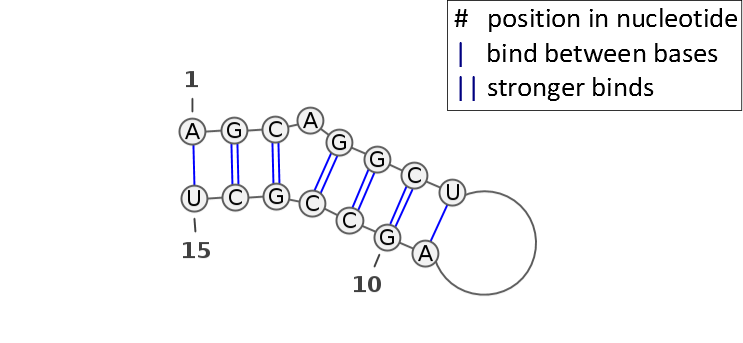
\includegraphics[scale=0.4]{./lib/bulge.png}
\caption{The RNA sequence {\tt AGCAGGCUAGCCGCU}. Note the bulging {\tt A} at position 4.}
\label{fig:bulge}
\end{figure}~
\\
\subsubsection{Interior Loop}
An interior loop occurs when two or more opposing bases are not complementary and 
can not bond, causing them both to bulge. This occurs when one or more 
consecutive bases mutate to another base. Figure~\ref{fig:int-loop} shows an interior 
loop.
\begin{figure}[h!]
\centering
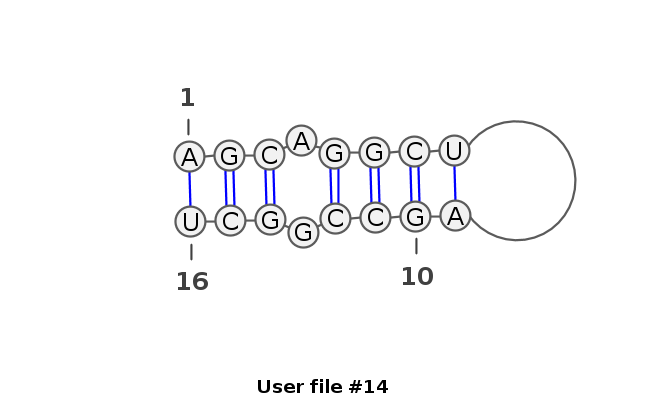
\includegraphics[scale=0.4]{./lib/interior-loop.png}
\caption{The RNA sequence {\tt AGCAGGCUAGCCGGCU}. Note the bulging {\tt A} at position 4 and {\tt G} at position 13
creating a loop inside the bonded strand.}
\label{fig:int-loop}
\end{figure}\\
These interior loops vary in size, and can have differing amount of bases on 
either side of the strands.
\subsubsection{Stem Loop}
A stem loop, also known as a hairpin loop, occurs when a strand bonds with 
itself, but leaves a sequence of bases sticking out, which does not bond with anything. 
This kind of loop occurs typically in RNA as they are single-stranded, but may 
happen in single stranded DNA. Figure~\ref{fig:stem-loop} 
shows a stem loop.
\begin{figure}[h!]\centering
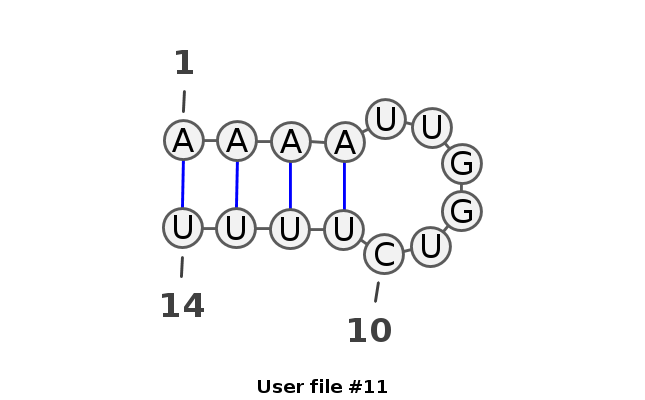
\includegraphics[scale=0.35]{./lib/stem-loop.png}
\caption{A stem loop of the RNA sequence {\tt AAAAUUGGUCUUUU}.}
\label{fig:stem-loop}
\end{figure}\\
An important thing to note is how the sequence can be seen as one 
long strand that starts from the adenine bases, which binds with the uracil bases, 
loops around without binding to anything and finally become the uracil bases 
which binds with the adenine bases from the beginning. This means that the 
stem loop from Figure~\ref{fig:stem-loop} can be written as one continuous 
sequence of bases; {\tt AAAAUUGGUCUUUU}. Since we can define a stem loop, we can 
search through a file documenting the bases of a nucleic acid and find all stem 
loops.

\documentclass[11pt,twoside,a4paper]{article}
\usepackage{pbox}
\usepackage{amsthm}
\newtheorem{definition}{Definition}
\newtheorem{example}{Example}
\begin{document}
\subsection{Scan\_For\_Matches}
Scan\_for\_matches is a string-searching tool created by Ross Overbeek, David 
Joerg and Morgan Price in C which searches through FASTA text files. Users specify 
what they wish to search for by defining a pattern, and scan\_for\_matches 
returns all matches that corresponds to the specified pattern.
\begin{definition}\label{patd}
A pattern is defined as follows:\\
\begin{tabular}{|r|l|}
\hline
{\tt ACUG}&Match the sequence ACUG\\
\hline
{\tt 1...5}&Match 1 to 5 characters\\
\hline
{\tt 3...3}&Match exactly 3 characters\\
\hline
{\tt p1=1...5}&Match 1 to 5 characters, and call the sequence p1\\
\hline
{\tt p1 $|$ p2}&Match either p1 or p2\\
\hline
{\tt p1[1,0,0]}&Match p1, allowing for one mismatch\\
\hline
{\tt p1[0,1,0]}&Match p1, allowing for one deletion\\
\hline
{\tt p1[0,0,1]}&Match p1, allowing for one insertion\\
\hline
{\tt length(p1+p2) $<$ 5}&The combined length of p1 and p2 must not exceed 4\\
\hline
{\tt r1=\{AB, BA\}}&\pbox{20cm}{Create a pattern rule where A is the complement of B, \\and B is the complement of A, and call it r1}\\
\hline
{\tt $<$p1}&Match the reverse of p1\\
\hline
{\tt \textasciitilde p1}&\pbox{20cm}{Match the reverse complement of p1 using the G-C, \\C-G, A-T and T-A pairing rule}\\
\hline
{\tt r1\textasciitilde p1}&\pbox{20cm}{Match the reverse complement of p1 using r1 rules}\\
\hline
{\tt \textasciicircum ~p1}&\pbox{20cm}{Match only p1 if it is at the start of a string}\\
\hline
{\tt p1 \$}&Match only p1 if it is at the end of a string\\
\hline
\end{tabular}
\end{definition}

\begin{definition}\label{patc}
Let {\tt E} be any pattern that's in the alphabet $\Sigma$ as defined in Definition \ref{patd}. 
Let $\epsilon$ be the empty string.
Let {\tt A} be a string that we are processing to see if the pattern is valid.
A pattern may then be constructed as such: \begin{center}
{\tt A = A' A | $\epsilon$}\\
{\tt A' = E}\end{center}
\end{definition}
Definition \ref{patc} states that a pattern may be any combination of the alphabet 
defined in definition \ref{patd}.
Using these patterns, it is possible to make very specific or very broad 
searches in a text file. 

\begin{example}
Say we want to write a pattern that finds the sequence {\tt GUUC}, allowing 
one mismatch, followed by a random sequence which has a length between 3 and 5, 
followed by the reverse complement of the first sequence that we found. We can 
then write this as \begin{center}
{\tt p1=GUUC[1,0,0] 3...5 \textasciitilde p1}
\end{center}
\end{example}

\end{document}

%\section{Theory}
\section{Regular expressions} 
  To explain what a regular expression is, we must first introduce languages and alphabets. All literals will be written using the typewriter font, to distinguish 
\begin{mydef}\label{alph}
An alphabet $\Sigma$ is a finite set of letters.
\end{mydef}

\begin{mydef}\label{lang}
A language is a infinite set of strings, composed by letters from an alphabet $\Sigma$
\end{mydef}

\begin{myex}
If we have a DNA sequence string, the alphabet $\Sigma$ consists of the literals ${\tt\{t,g,c,a\}}$. and the language contains strings formed by the literals from this alphabet. For example "gtcaaa" or "gtcaaat". 
\end{myex}

\begin{mydef}
E is a regular expression(RE) if either:
\begin{itemize} 
\item E is a atomic expression, that consist of a letter from an alphabet $\Sigma$ or special character 1.
\item Given two RE's $E_1$ and $E_2$. E is a compound expression formed by $E_1 + E_2$, $E_1 E_2$ or $E_1 ^*$ 
\end{itemize}
\end{mydef}



\begin{mydef}
A regular expression is described by the following grammar: \\
\begin{center}
$E::= a|1|E_1 + E_2 |E_1 E_2 | E^* | 0$
\end{center}
where $E_1$ and $E_2$ are RE's and $a \in \Sigma$
\end{mydef}

\begin{mydef}\centering
The language interpation of L(E) of a regular expression is: 
\begin{align*}
L(0)           &= \emptyset\\
L({\tt a})     &= \{{\tt a}\} \\
L(1)         &= \{\epsilon\} \\
L(E_0 + E_1) &= L(E_0) \cup L(E_1) \\
L(E_1 E_2)   &= \{w_1w_2 | w_1 \in L(E_1),w_2 \in L(E_2)\}=L(E_1)L(E_2) \\
L(E^*)       &= \bigcup\limits_{n=0}^\infty L(E)^n 
\end{align*}
%\cite[p.5 def. 3]{crash}
\end{mydef}

With definition 2, we can now form regular languages. For example, natural numbers described as a regular expression. Natural numbers have the alphabet $\Sigma$ = \{{\tt 0,1,2,3,4,5,6,7,8,9}\}, the regular expression for natural numbers would look like:
\begin{center}
$E_{nat} = $(1+2+3+4+5+6+7+8+9)(0+1+2+3+4+5+6+7+8+9)$^*$
\end{center}

\section{Nondeterministic Finite Automaton}
\begin{mydef}
An nondeterministic finite automaton (NFA) is a 5-tuple $(Q,\Sigma,\Delta,q^s ,q^f)$. Where $Q$ is a finite set of states,$\Sigma$ is the input alphabet, the initial state $q^s \in Q$,  the accepting state $q^f \in Q$ and $\Delta$ is the set that contains all the transitions. Transitions in $\Delta$ is shown $q^1\xrightarrow{a}q^2$ where $q^1\in Q,q^2\in Q$ and the label $a$ is either $a \in \Sigma$ or  the empty transition $\epsilon$
\end{mydef}

\subsection{Conversion from RE to NFA}
\label{RA_TO_NFA}
One of the main reasons for using NFAs when working with regular expressions is the direct correlation between regular expressions and NFAs. Each expression can be converted to an NFA, and vice versa. Table~\ref{tab:NFA_TAB} shows the correlation between regular expressions and NFA for the most common expressions.
%\\
%(( NOTE: We'll include a table with conversions ))
%\\
%With little effort every regular expression can be translated into a graph, which can then be analysed.

\begin{table}[h!]
\caption{Translation table from regular expressions to NFA}
\centering
\begin{tabular}{*{2}{m{0.4\textwidth}}}
\hline
\begin{center}$a$\end{center} &\begin{center} 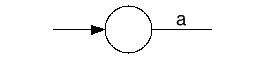
\includegraphics[width=0.25\textwidth]{lib/dot/a.png} \end{center} \\
\hline
\begin{center}$\epsilon$\end{center} &\begin{center} 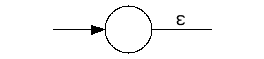
\includegraphics[width=0.25\textwidth]{lib/dot/epsilon.png} \end{center} \\
\hline
\begin{center}$ab$\end{center} &\begin{center} 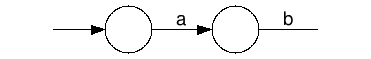
\includegraphics[width=0.3\textwidth]{lib/dot/ab.png} \end{center} \\
\hline
\begin{center}$a\vert b$\end{center} &\begin{center} 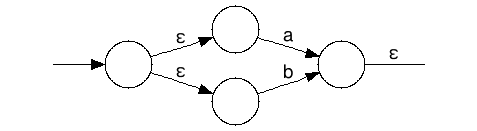
\includegraphics[width=0.35\textwidth]{lib/dot/a-or-b.png} \end{center} \\
\hline
\begin{center}$a^*$\end{center} &\begin{center} 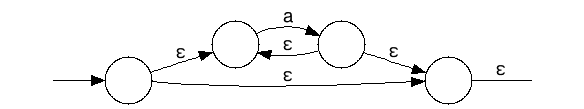
\includegraphics[width=0.4\textwidth]{lib/dot/a_star.png} \end{center} \\
\hline
\end{tabular}
\label{tab:NFA_TAB}
\end{table}

%
%\begin{figure}[h!]
 % \centering
%\begin{minipage}[b]{0.40\linewidth}
 % \centering
   %   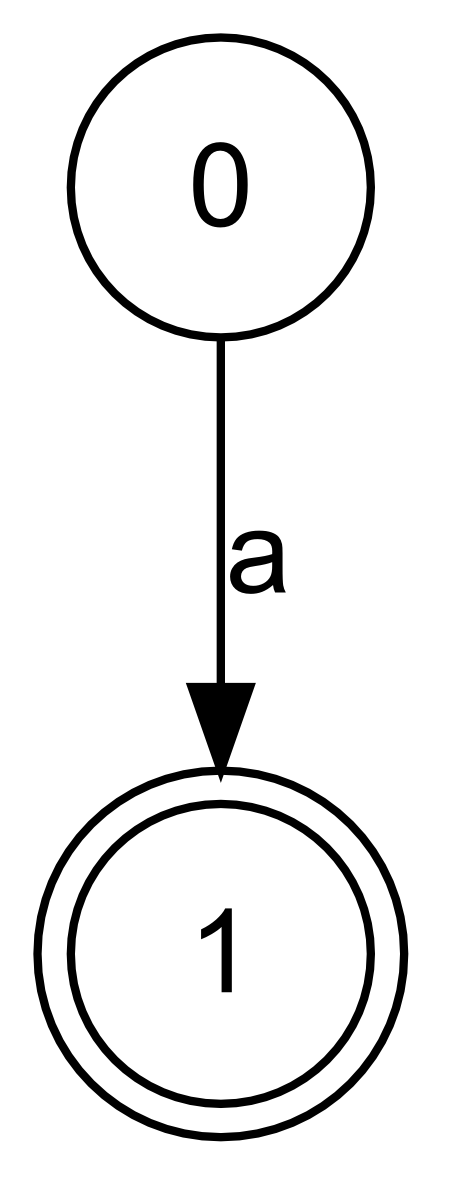
\includegraphics[width=0.2\textwidth]{lib/A.png}
  %\caption{NFA of the expression $a$}
%\label{fig:A}
%  \end{minipage}
%\begin{minipage}[b]{0.40\linewidth}

%  \centering
   %   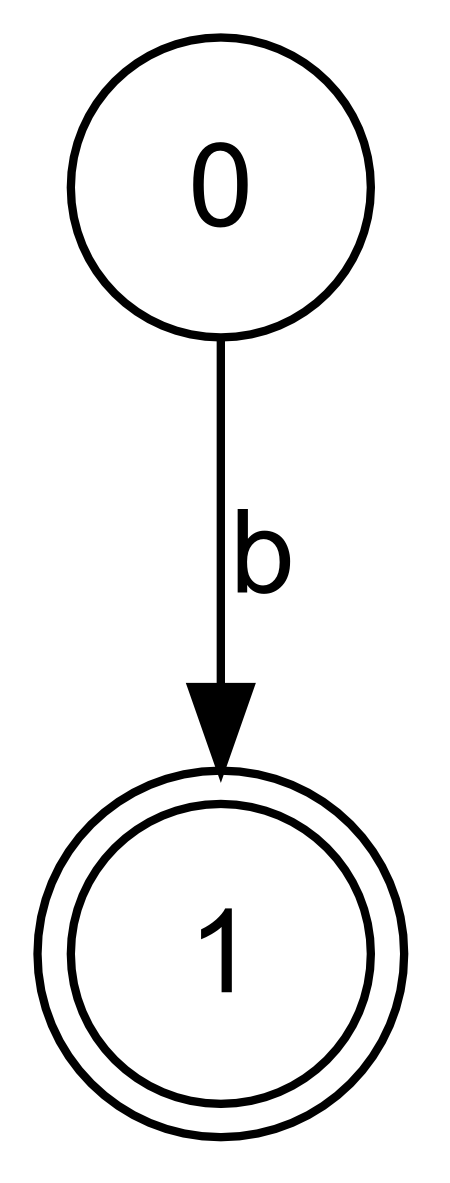
\includegraphics[width=0.2\textwidth]{lib/B.png}
  %\caption{NFA of the expression $b$}
  %\label{fig:B}
%    \end{minipage}
%\end{figure}

%For example two NFAs of regular expression $a$ and $b$ will appear as shown in Figure~\ref{fig:A} \& \ref{fig:B}, each of them starts in node $0$ and ends in node $1$, and these nodes are connected by a one-way transition with a value $a$ or $b$. %, it may be worth noting that our implementation always converts to lower case when constructing and matching.

%To construct the NFA for $A | B$ , one will first have to construct an NFA for both $A$ and $B$, which will then be combined, making the full NFA. The $|$ operator this is achieved by constructing two new nodes, the first having epsilon-transition pointing to the start node of each of the two NFAs $A$ and $B$, then for each NFA $A$ and $B$ the ending node will instead of ending the NFA, have a new epsilon-transition to the second new node, in the figure below, Figure~\ref{fig:A_OR_B}, the two new nodes are labeled $0$ and $5$:

%\begin{figure}[h!]
 % \centering
   %   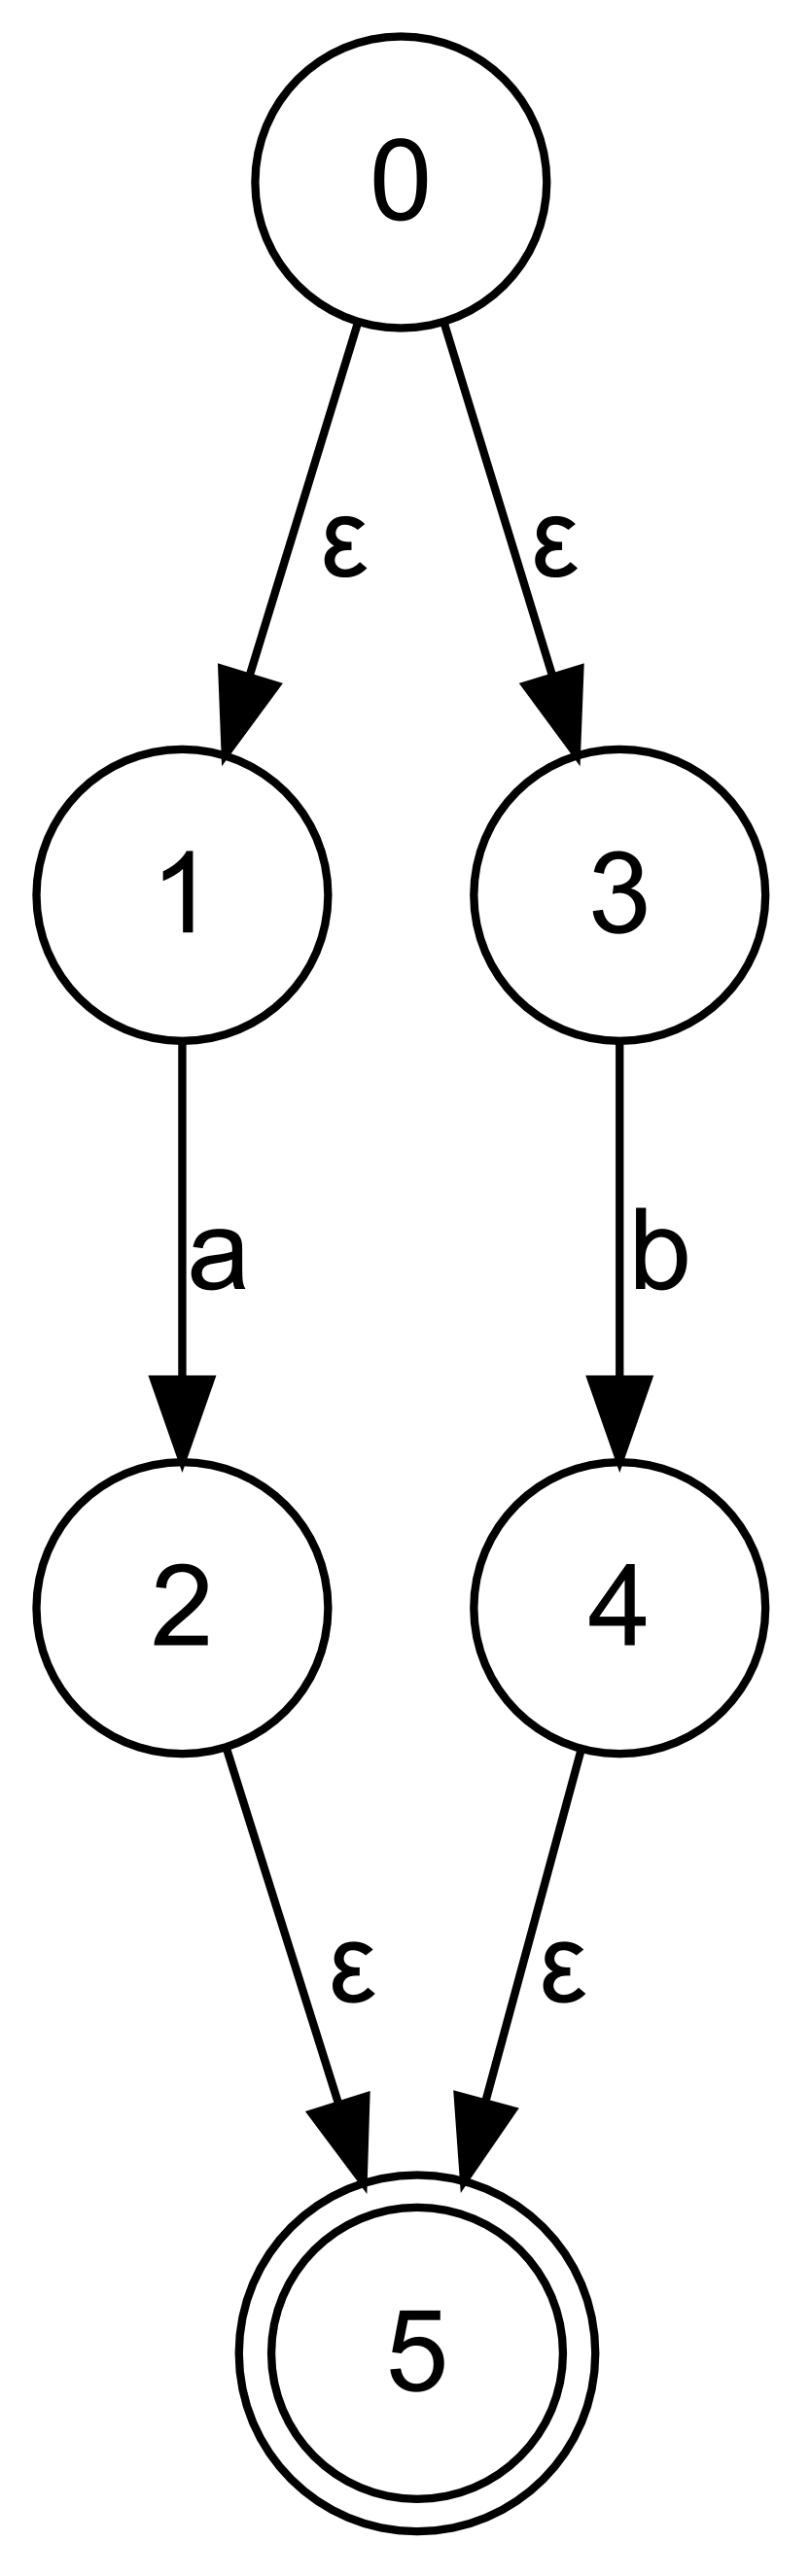
\includegraphics[width=0.1\textwidth]{lib/A_OR_B.png}
 % \caption{NFA of the expression $a | b$}
%\label{fig:A_OR_B}
%\end{figure}

Once a NFA-structure has been build, we can start matching a text against the NFA.

This is achieved by having a set of states, each state is looking at a node in the structure, while keeping track of previous nodes traversed by the state. Whenever a new character is being checked to match, each state will look at its node, and determine if it's possible to accept the character in the NFA, either by taking a transition labeled with the character, or alternatively via an epsilon-transition. When two possible transitions are viable, new states will be created in the set of states, so that each possible transition will be explored.

Any state that will fail to match the character will be removed from the set of states.
%\begin{figure}[h!]
 % \centering
%\begin{minipage}[b]{0.40\linewidth}
 % \centering
   %   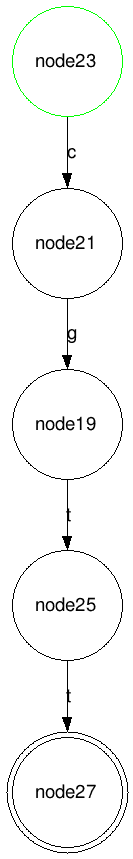
\includegraphics[width=0.2\textwidth]{lib/cgtt1.png}
   % \caption{NFA of $CGTT$, with a state looking at node23.\\}
    %\label{fig:CGTT_1}
 % \end{minipage}
%\begin{minipage}[b]{0.40\linewidth}
%\centering
%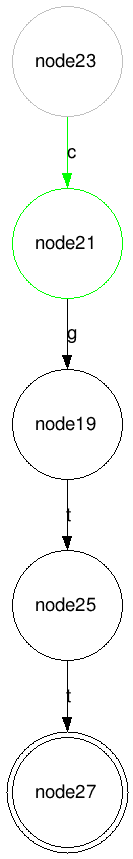
\includegraphics[width=0.2\textwidth]{lib/cgtt2.png}
% \caption{Next iteration of the state on Figure~\ref{fig:CGTT_1}, the state is now in node21.}
  %  \end{minipage}
%\label{fig::cgtt}
%\end{figure}

Only if a state reaches the ending node of the NFA, there's a match.

\newpage

\subsection{Insertions, Deletions and Mutations}
NFAs do not support mismatching by default, although a regular expression can be built to handle mismatches. While doing handling mismatching while constructing the regular expression, we are interested in having an NFA, and allowing matching while with support for insertions, deletions and mutations, hence we need to define a way to handle this.

We can do this by adding a counter for insertions, deletions and mutations, and when a transition is not possible in the NFA, we decrease these counters and preform alternative transitions to emulate these conditions.
%Currently our implementation supports a simple solution to the insertion, deletion and mutation problem, which is achieved by having a counter for insertions, deletions and mutation in each state, these counters symbolise the number of allowed occurrences of each mutation, insertion and deletion.
\begin{description}
\item[] For insertions, the state will remember the unmatched character, but the state won't move from its current node.
\item[]For deletions, the state wont remember the unmatched character, but it will take every transition going on from the node.
\item[] For mutations, the same happens as in a deletion, but now the state also remembers the unmatched character.
\end{description}
Figure~\ref{fig:ins_mut_del} illustrates how states move through a NFA when mismatches occur. 

\begin{figure}[h!]
  \centering
      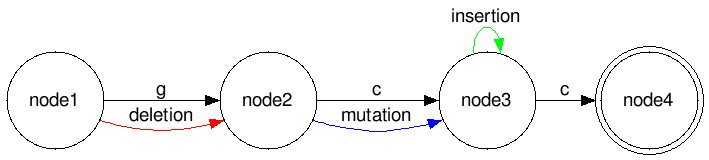
\includegraphics[width=0.6\textwidth]{lib/gcc_ins_mut_del.png}
  \caption{Simple NFA of $GCC$, showing behaviour of insertion, mutation and deletion}
\label{fig:ins_mut_del}
\end{figure}
%Depending on the number of insertions, deletions and mutations allowed, this approach will grant each state a much longer lifespan, and for each non-matching character parsed, one state may turn into three, which all needs to be processed for each new character parsed, resulting in an increasingly slower running time as the allowed number of insertions, deletions and mutations increase, but it does give us the utility that we require.
%\label{state:insertion1}


%In the next iteration of our implementation, we aim to implement levenstein automations\cite{WikiLevenshtein}, which hopefully will help speed up the runtime, and also, currently our solution will work on any given regular expression, thus a logical step which also may deliver some increase in performance would be to enforce a constriction such that it only allows for a RNA language similar to that defined in Section~\ref{section:RE}.
%\section{Method}

%\section{Conclusion}
\newpage
\nocite{*}
\bibliographystyle{unsrt}
\bibliography{./References/references.bib}
\end{document}